\documentclass[a4paper,12pt,twoside,titlepage]{article}

%Additional packages
\usepackage[utf8]{inputenc}
\usepackage[T1]{fontenc}
\usepackage[dutch,english]{babel}
\usepackage{syntonly}
\usepackage[official]{eurosym}
\usepackage{csquotes}

% Handle images
\usepackage{graphicx}
\graphicspath{ {./images/}{./styles/} }
\usepackage{float}
\usepackage{wrapfig}

% Handle URLs
\usepackage{xurl}
\usepackage{hyperref}
\hypersetup{colorlinks=true, linkcolor=blue, citecolor=blue, filecolor=blue, urlcolor=blue, pdftitle=, pdfauthor=, pdfsubject=, pdfkeywords=}

% Tables and listings
\usepackage{multirow,tabularx}
\usepackage[table]{xcolor} % Table colors
\usepackage{scrextend}
\addtokomafont{labelinglabel}{\sffamily}
\usepackage{listings}
\usepackage{adjustbox}

% Turn on indexing
\usepackage{imakeidx}
\makeindex[intoc]

% Define colors
\usepackage{color}
\definecolor{ashgrey}{rgb}{0.7, 0.75, 0.71}




% Listing style
\lstset{
  backgroundcolor=\color{ashgrey}, % choose the background color; you must add \usepackage{color} or \usepackage{xcolor}; should come as last argument
  rulecolor=\color{black},         % if not set, the frame-color may be changed on line-breaks within not-black text (e.g. comments (green here))
  frame=single,	                   % adds a frame around the code
  basicstyle=\footnotesize\ttfamily,  	   % the size of the fonts that are used for the code
  extendedchars=true,    	   % lets you use non-ASCII characters; for 8-bits encodings only, does not work with UTF-8
  breakatwhitespace=true, 	   % sets if automatic breaks should only happen at whitespace
  breaklines=true,        	   % sets automatic line breaking
  keepspaces=true,        	   % keeps spaces in text, useful for keeping indentation of code (possibly needs columns=flexible)
  columns=fullflexible,	  	   % Make sure no extra spaces are added.
  showstringspaces=false, 	   % if true show spaces in strings adding particular underscores
  showspaces=false        	   % show spaces everywhere adding particular underscores; it overrides 'showstringspaces'
}



\lstdefinestyle{DOS}
{
    backgroundcolor=\color{black},
    basicstyle=\scriptsize\color{white}\ttfamily
}

% Uncomment for production
% \syntaxonly

% Style
\pagestyle{headings}

% Define document
\author{D. Leeuw}
\title{Windows: Troubleshooting}
\date{\today\\
0.0.0
\vfill
\raggedright
\copyright\ 2025 Dennis Leeuw\\

%\begin{figure}

\includegraphics[width=0.3\textwidth]{CC-BY-SA-NC.png}
%\end{figure}

Dit werk is uitgegeven onder de Creative Commons BY-NC-SA Licentie en laat anderen toe het werk te kopi\"eren, distribueren, vertonen, op te voeren, en om afgeleid materiaal te maken, zolang de auteurs en uitgever worden vermeld als maker van het werk, het werk niet commercieel gebruikt wordt en afgeleide werken onder identieke voorwaarden worden verspreid.


}


\begin{document}
\selectlanguage{dutch}

\maketitle

%%%%%%%%%%%%%%%%%%%
%%% Introductie %%%
%%%%%%%%%%%%%%%%%%%

%%%%%%%%%%%%%%%%%
%%% De inhoud %%%
%%%%%%%%%%%%%%%%%

% requires: 
% provides: 

\section{Introductie}
Zoals je zult begrijpen is het niet mogelijk om in \'e\'en document alle problemen die kunnen voorkomen in een besturingssysteem te behandelen. We zullen in dit document dan ook een aantal algemene richtlijnen geven die je kunnen helpen bij het oplossen van problemen met Windows.



\section{Boot problems}
Het kan gebeuren dat je systeem helemaal niet meer wil opstarten. Dit kan aan de hardware liggen of aan de software. Voordat je iets gaat doen, controlleer eerst alle kabels. Doorloop de volgende stappen om het probleem te detecteren:
\begin{enumerate}
\item Als je computer aan zet gaat dan het power-ledje branden, zo nee dan is er waarschijnlijk geen spanning
	\begin{enumerate}
	\item Controlleer of er spanning zit op de wandcontactdoos waar de computer in zit (Gebruik een spanningsmeter)
	\item Controlleer of er een kabel stuk is (vervang door een bekende goede kabel)
	\end{enumerate}
\item Hoor je piepjes uit je computer komen en is er geen beeld op het beeldscherm? (je hebt spanning, er iets niet goed met de hardware)
	\begin{enumerate}
	\item Noteer het aantal piepjes en zoek op Internet naar de handleiding van je moederbord en zoek op wat de piepjes betekenen.
	\end{enumerate}
\item Hoor je geen piepjes, je hebt wel beeld: wat is de error melding op het scherm
	\begin{enumerate}
	\item Zoek de error melding op op het Internet met een andere computer (telefoon)
	\end{enumerate}
\end{enumerate}


\section{Herstel het MBR}
Herstel de master boot record (MBR)
\begin{enumerate}
\item Boot van een Windows CD (installatie CD)
\item Settings app -> Update \& Security -> Recovery -> Advanced Startup
\item Troubleshoot -> Advanced Options -> Command Prompt 
\item \texttt{bootrec /RebuildBcd}
\item \texttt{bootrec /fixMbr}
\item \texttt{bootrec /fixboot}
\item \texttt{exit}
\item Verwijder CD en reboot.
\end{enumerate}


\section{Het lezen van de logs}
De logs zijn stukjes tekst die een systeem genereert op basis van gebeurtenissen. Als er bijvoorbeeld een gebruiker inlogt kan het systeem een bericht (log) genereren dat de gebruiker succesvol is ingelogd.

Een systeem maakt verschillende soorten log berichten aan. De berichten kunnen gaan over het systeem, over de beveiliging of over applicaties. Als er een probleem is met het besturingssysteem of een applicatie is Event Viewer vaak de eerste plek om te gaan zoeken.

De logs bevatten informatie over wat er gebeurd is en de datum en het tijdstip waarop de gebeurtenis heeft plaatsgevonden. Ook kunnen ze foutcodes bevatten waarop je op Internet kunt zoeken naar meer informatie en mogelijke oplossingen.

Om deze logs te kunnen bekijken is er een MMC-module met de naam Event Viewer\index{event viewer}\index{mmc!event viewer} (Logboeken\index{logboeken}\index{mmc!logboeken}. Met Event Viewer kan je ook logs beheren.

Binnen Event Viewer ...
is ingedeeld in categorieën zoals Windows-logboeken, toepassings- en serviceslogboeken en abonnementen. Gebruikers kunnen logboeken filteren op criteria zoals gebeurtenisniveau, datum en trefwoorden om snel relevante gebeurtenissen te vinden. Met de Logboeken kunnen gebruikers ook logboekbestanden opslaan voor analyse en gebeurtenisgegevens exporteren voor extern gebruik.

Voor IT-professionals is de Logboeken een krachtig hulpprogramma voor het diagnosticeren van problemen, het controleren van systeemactiviteiten en het garanderen van naleving van beveiligingsbeleid. Het wordt ook gebruikt om de status en status van servers en andere kritieke infrastructuuronderdelen bij te houden.

Om Event Viewer te openen zijn er verschillende manieren:
\begin{itemize}
\item
	\begin{enumerate}
		\item Start MMC
		\item Selecteer in het File menu Add/Remove snap-in
		\item Selecteer Event Viewer en klik op Add
	\end{enumerate}
\item Gebruik de windows-toets + r en run eventvwr.msc\index{eventvwr.msc}
\item Klik op het zoek icoon en zoek op Event Viewer
\end{itemize}

%% \begin{minipage}[t]{\linewidth}
%% \raggedright
%% \adjustbox{valign=t}{%
%% 	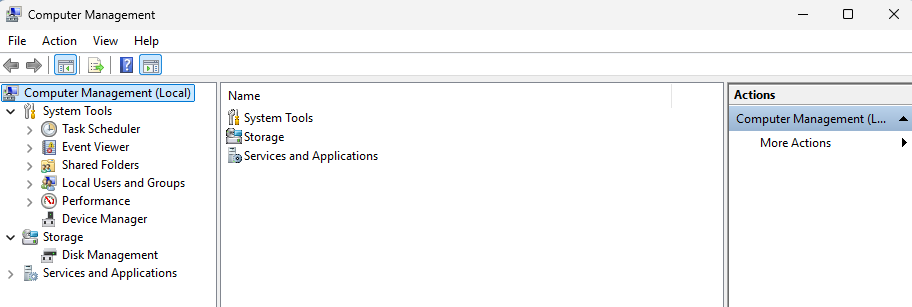
\includegraphics[width=0.99\linewidth]{computermanagement.png}%
%% }
%% \end{minipage}


\subsection{Event Viewer Logboeken}
Na het openen van Event Viewer heb je een aantal mappen waaruit je kunt kiezen:
\begin{description}
\item[Custom Views] Speciale views die je zelf niet kunt maken.
\item[Windows Logs] De log die gemaakt worden alles wat met het besturingssysteem Windows te maken heeft.
\item[Applications and Services Logs] Logs die gemaakt worden door applicaties en services die geen onderdeel van Windows zijn.
\item[Subscriptions] 
\end{description}
Binnen deze mappen vind je de logboeken. Logboeken bestaan uit gebeurtenissen (Events) die gelogd zijn door de software en die vast gelegd zijn met een datum en tijd. In de rest van dit hoofdstuk kan we deze verschillende mappen nader bekijken.


In Event Viewer heeft Windows zijn eigen map om in te loggen. Alle gelogde events die met het operating system te maken hebben komen in deze map terecht. Als we dus willen weten hoe het is met Windows is dit de juiste plek om dat te onderzoeken. De zaken die te maken hebben met veiligheid zijn te vinden in de \texttt{Security} map.


\subsection{Event Viewer Events}
Als we binnen Event Viewer naar de \textquote{Windows Logs} gaan en daar klikken op \textquote{System} dan zien we er alle meldingen van het systeem die vastgelegd zijn. Dubbelklikken we op een Event dan krijgen we meer uitgebreidde informatie.

\begin{minipage}[t]{\linewidth}
\raggedright
\adjustbox{valign=t}{%
	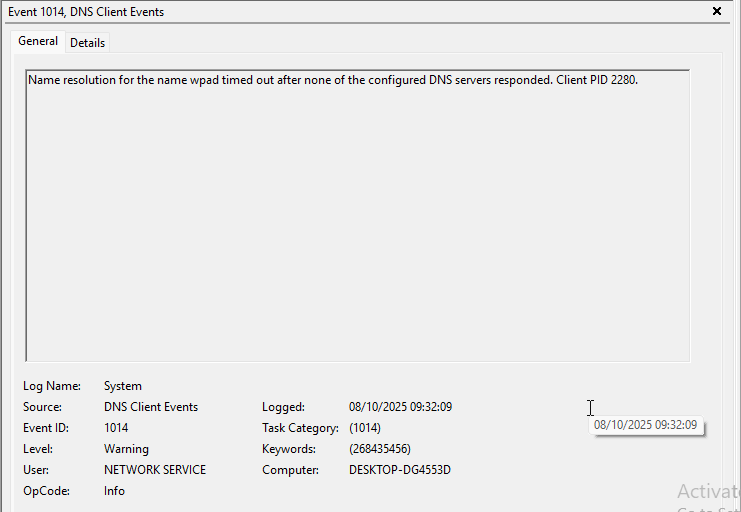
\includegraphics[width=0.99\linewidth]{ev-event.png}%
}
\end{minipage}

Bij dit event zien we een aantal verschillende velden onder de mededeling. Een aantal van deze velden zijn voor ons van belang:
\begin{description}
\item[Logged] geeft de datum en tijd waarop het event is binnengekomen
\item[Source] vertelt ons iets over de herkomst van het event
\item[Event ID] is een nummer dat ons kan helpen bij het vinden van nadere informatie. Via een Internet Zoekmachine kunnen we zoeken op de Event ID en zo meer informatie verzamelen over het gebeurde. Het beste is om te zoeken naar \textquote{Windows Event ID <nummer>}
\item[Level] geeft aan hoe belangrijk een event is. Er zijn verschillende levels:
	\begin{description}
	\item[Critical] Dit zijn meldingen waarop direct gereageerd zou moeten worden.
	\item[Error] Problemen die optreden, maar die kritiek zijn.
	\item[Warning] Waarschuwingen die een indicatie kunnen zijn dat er een probleem zit aan te komen. Zouden nader onderzocht moeten worden om problemen voor te zijn.
	\item[Information] Informatie die handig is om te weten, maar die geen probleem aangeven.
	\item[Verbose] Informatie die voortgang of succes meldingen zijn. Kunnen over het algemeen genegeerd worden.
	\end{description}
\end{description}


\subsection{Filtering Logs}
De lijsten met events kunnen behoorlijk lang zijn in Event Viewer. Het zou makkelijker zijn als we alleen de belangrijke events kunnen zien, bijvoorbeeld alleen Critical en Error. En gelukkig kan dat ook in Event Viewer.

\begin{minipage}[t]{\linewidth}
\raggedright
\adjustbox{valign=t}{%
	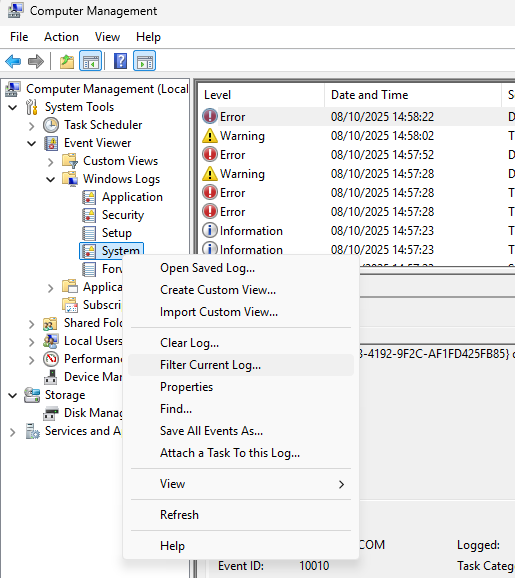
\includegraphics[width=0.99\linewidth]{ev-filter.png}%
}
\end{minipage}

Door rechts te klikken op het logboek kan je \textquote{Filter Current Log...} selecteren. In het nieuwe venster is het mogelijk om te filteren op Event level.



\section{Storage problems}
\subsection{Disk Management}
In de Computer Management applicatie vind je onder Storage een kopje Disk Management. Daar kunnen we informatie opvragen over onze disks.

\begin{minipage}[t]{\linewidth}
\raggedright
\adjustbox{valign=t}{%
   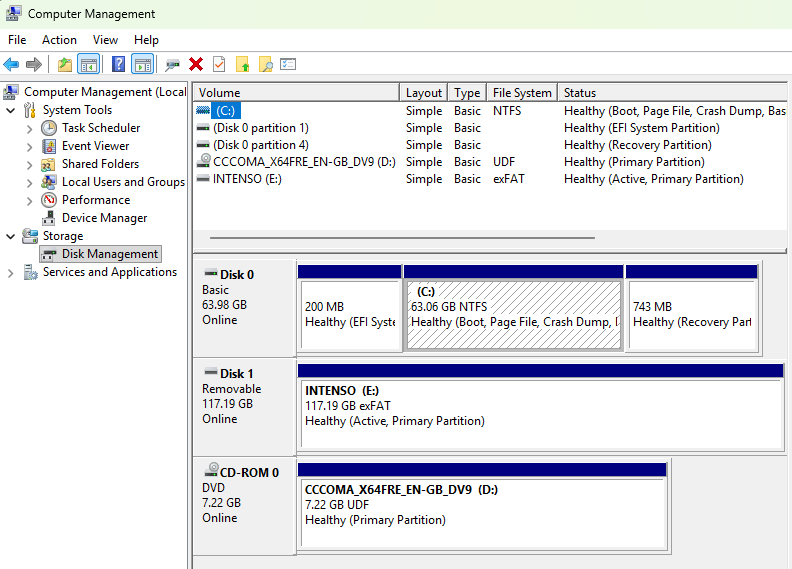
\includegraphics[width=0.99\linewidth]{computer_management-disks.png}%
}
\end{minipage}

We zien in het plaatje een harddisk (Disk 0), een USB-stick (Disk 1) en een DVD (CD-ROM 0). We zien tevens dat ze allemaal gebruik maken van een ander filesystem. De partitie op de harddisk die onze C: drive is gebruikt NTFS, de USB-stick exFAT en de DVD UDF.
\begin{description}
\item[UDF] Universal Disk Format: Een bestandssysteem dat veel gebruikt wordt voor media die \'e\'en keer geschreven worden en daarna alleen gelezen. Je komt dit tegen op data CD's en DVD's. UDF is een extensie en de opvolger van ISO-9960. Als we praten over een ISO-image dan bedoelen we tegenwoordig vaak UDF.
\item[exFAT] extensible File Allocation Table: is de opvolger van FAT het bestandssysteem dat door Microsoft gebruikt wordt sinds DOS. exFAT ontwikkeld door Microsoft en is simpel en open source. Er is ondersteuning voor exFAT in Windows, Linux en MacOS X, daarmee is het het ideale bestandssysteem om data uit te wisselen tussen verschillende systemen. Je komt het dan ook vaak tegen op USB-sticks.
\item[NTFS] New Technology File System: Een door Microsoft ontwikkeld bestandssysteem dat gebruikt wordt vanaf Windows NT. Het is een relatief complex bestandssysteem dat veel extra data (META-data) kan bijhouden. Die metadata bestaat voornamelijk uit wie welke rechten heeft op de bestanden en directories.
\end{description}

In het Volume overzicht zien we onze C: drive. Gebruiken we de rechermuisklik op deze drive dan krijgen we een menutje waaruit we Properties kunnen selecten. Properties bestaat uit verschillende tabs:
\begin{description}
\item[General] geeft een overzicht van het gebruik van de disk. Een klik op details brengt je naar Settings, System Storage, Show more categories.
\item[Hardware] Geeft je meer specieke informatie over een drive, via deze ingang kan je ook driver updates doen voor een drive.
\item[Security] Hierin kan je zetten wie er welke rechten heeft op de partitie.
\item[Sharing] Hier kan je je disk delen met andere gebruikers of systemen op het netwerk.
\item[Quota] Hier kan je quota zetten. Dit is standaard gedisabled. Via het knopje \textquote{Quota Entries} kan je per gebruiker aangeven hoeveel diskspace deze mag gebruiken. Dat is de quota per gebruiker.
\item[Previous Versions] is een overzicht van oude restore points
\item[Tools] Bevat de tools Error checking en Optimise and defragmentation drive. Deze onderdelen worden in volgende secties behandeld.
\end{description}


\subsection{Error Checking}
Error checking controleert je disk op fouten.

Je kan de controle ook op de commandline doen. Start daarvoor PowerShell op als Administrator en run:
\begin{lstlisting}[language=bash]
sfc /scannow
\end{lstlisting}
De \texttt{sfc} (System File Checker) tool scant de disk op errors. Mochten deze er zijn dan kan je met \texttt{dism} (Deployment Image Servicing and Management) proberen de problemen op te lossen:
\begin{lstlisting}[language=bash]
dism /online /cleanup-image /restorehealth
sfc /scannow
\end{lstlisting}

Treden er na de tweede scan van \texttt{sfc} geen errors meer op, reboot dan Windows en alles zou weer goed moeten zijn.


\subsection{Defragmentation}
Met de moderne SSDs is defragmentation niet meer nodig, sterker het zou je SSD sneller kunnen doen verouderen. Als je nog een harddisk gebruikt legt deze sectie je uit wat defragmentation is en waarom je het nodig hebt.

Defragmentatie is het netjes achter elkaar leggen van sectoren die behoren bij een bestand. Een harddisk is ingedeeld in sectoren (van bijv. 512 bytes). Elk bestand wordt opgehak in stukjes die in een sector passen en dan weggeschreven. Het filesystem houdt in een tabel bij welke sectoren er bij welk bestand horen en in welke volgorde ze gelezen moeten worden. Ideaal is het als alle data netjes op een cylinder ligt en alle sectoren netjes naast elkaar. Dan hoeft de leeskop het minst te bewegen en kan er de maximale hoeveelheid data gelezen worden.

Tijdens het gebruik van een harddisk worden er bestanden geschreven, verwijderd en bestanden worden groter of kleiner. Dit betekent dat data niet altijd meer op de ideale plek op de harddisk terecht komt. Als een bestand bijvoorbeeld groter wordt kan het zijn dat de eerste 100k keurig op de harddisk ligt maar dat de laatste 50k verspreid is geraakt over verschillende sectoren/cylinders. Dit heet fragmentatie.

Bij defragmentatie wordt de data weer op de ideale manier over de harddisk verspreid, waardoor er snelheidswinst bereikt kan worden. Defragmentatie is niet een eenmalige handeling, deze moet regelmatig herhaald worden.

\begin{minipage}[t]{\linewidth}
\raggedright
\adjustbox{valign=t}{%
   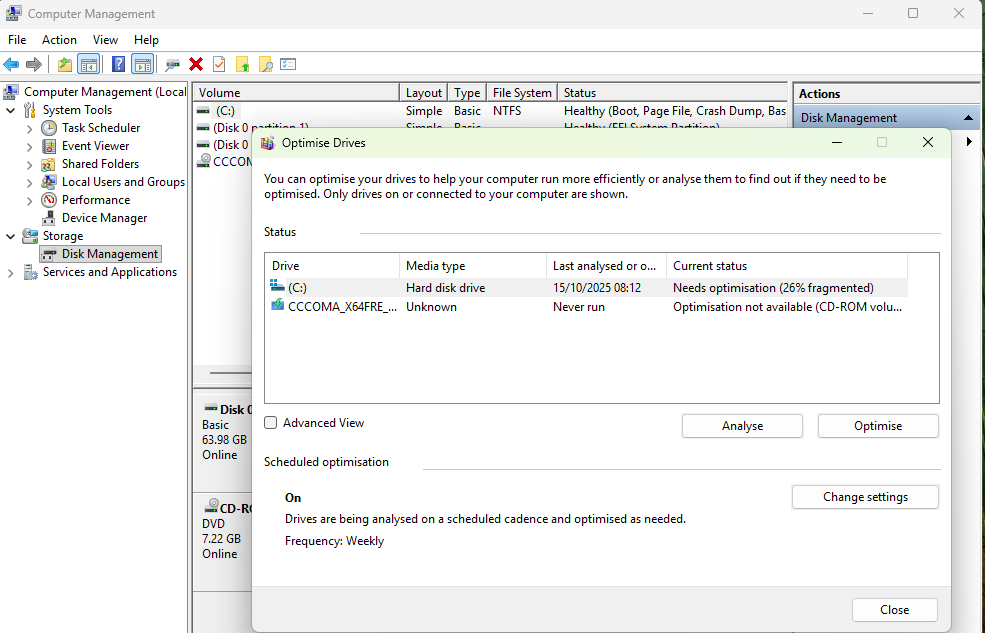
\includegraphics[width=0.99\linewidth]{computer_management-disks_defrag.png}%
}
\end{minipage}

SSDs hoeven niet gedefragmenteerd te worden omdat de toegang tot een SSD overal even snel is. Er is geen kop die verplaatst moet worden, dus je wint niets bij het defragmenteren. In het ergste geval wordt data ergens anders op de SSD weggeschreven en dat kost write-cycles wat slecht is voor een SSD.


\subsection{Disk Clean-Up}
Tijdens het gebruik van Windows worden er veel tijdelijke (cache) bestanden weggeschreven op de harddisk. Via Disk Clean-Up kan je hier opruiming in houden.

\begin{minipage}[t]{\linewidth}
\raggedright
\adjustbox{valign=t}{%
   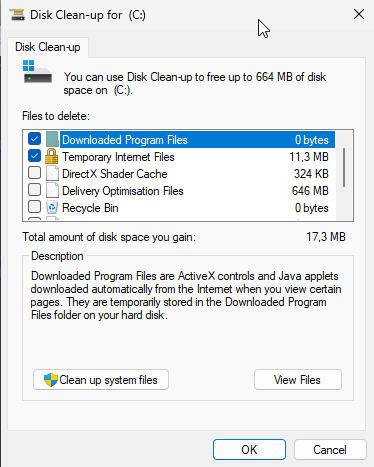
\includegraphics[width=0.75\linewidth]{disk_cleanup.png}%
}
\end{minipage}



\section{Network issues}

\section{Device problems}
\subsection{Keyboard en mouse}
\subsection{Monitor}
\subsection{Printers}

\section{Application problems}
\subsection{Application slow}
\subsection{Application frozen}

\section{Windows is frozen}

\section{Automatic Troubleshooting}
Windows kan terwijl jij erop werkt data over de status van je systeem naar Microsoft sturen. Op basis van deze data kan Microsoft adviezen uitbrengen over je systeem.

Hier moet je goed over nadenken. Hoeveel data over je systeem, de applicaties die je gebruikt en de sites die je bezoekt wil je met Microsoft delen in ruil voor goede adviezen over hoe je je systeem beter kunt beheren en fine-tunen.

Om je te laten zien waar je kan instellen wat je met Microsoft deelt en wat dat voor consequenties heeft. Starten we de Settings app op, gaan naar System en dan naar Troubleshoot. Hier kunnen we bij opties bepalen of automatische troubleshooters mogen draaien. De keuze bij de opties zijn:
\begin{itemize}
\item Run automatically, don't notify me
\item Run automatically, then notify me
\item Ask me before running (default)
\item Don't run any
\end{itemize}

\begin{minipage}[t]{\linewidth}
\raggedright
\adjustbox{valign=t}{%
	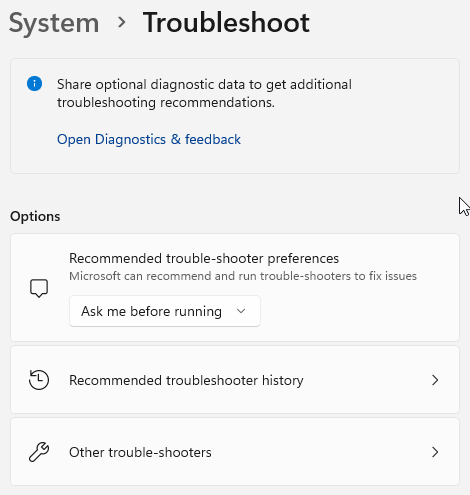
\includegraphics[width=0.99\linewidth]{settings_troubleshoot.png}%
}
\end{minipage}

Klikken we op \textquote{Open Diagnostics \& feedback} dan krijgen we nog veel meer opties die we kunnen instellen

\begin{minipage}[t]{\linewidth}
\raggedright
\adjustbox{valign=t}{%
	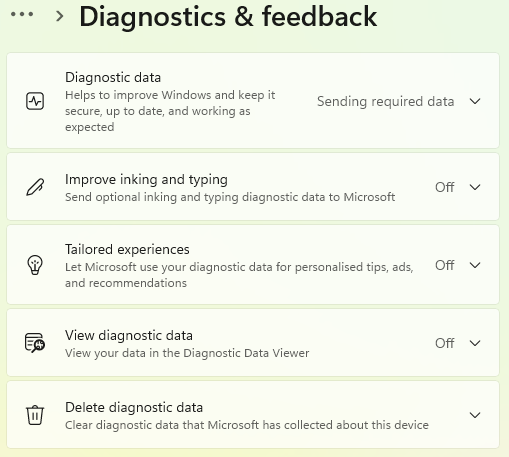
\includegraphics[width=0.99\linewidth]{settings-diagnostics_feedback.png}%
}
\end{minipage}

Loop door de verschillende items heen en kijk welke opties je aan of juist uit wil zetten.

Als we terug gaan naar de vorige pagina van de Troubleshoot settings, dan zien we dat er ook nog een kopje is met \textquote{Other trouble-shooters}. Hier kunnen we per onderdeel van ons systeem met hulp krijgen bij het onderzoeken van problemen met ons systeem.




%%%%%%%%%%%%%%%%%%%%%
%%% Index and End %%%
%%%%%%%%%%%%%%%%%%%%%
\printindex
\end{document}

%%% Last line %%%
